% --- Question 3 (1) のスライド ---
\begin{frame}{Question 3 (1): グラフのフォーマルな記述}
    \begin{columns}[c] % 左右分割の開始
        
        % 左側：画像（幅の40%）
        \begin{column}{0.4\textwidth}
            \centering
            % 画像ファイル名が正しいか確認してください
            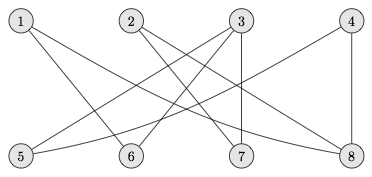
\includegraphics[width=\linewidth]{image/question3_matching.png}
            \vspace{1em}
            \small{グラフ $G_1$}
        \end{column}
        
        % 右側：テキスト（幅の60%）
        \begin{column}{0.6\textwidth}
            \begin{block}{問題 (1)}
                $G_1$ のフォーマルな記述を答えなさい．
            \end{block}
            
            \textbf{頂点集合 (Vertices):}
            \[ V_1 = \{1, 2, 3, 4, 5, 6, 7, 8\} \]
            
            \textbf{辺集合 (Edges):}
            \begin{align*}
                E_1 = \{ & \{1, 6\}, \{1, 8\}, \\
                         & \{2, 5\}, \{2, 7\}, \\
                         & \{3, 6\}, \{3, 8\}, \\
                         & \{4, 5\}, \{4, 8\} \}
            \end{align*}
        \end{column}
        
    \end{columns}
\end{frame}

% --- Question 3 (2) のスライド ---
\begin{frame}{Question 3 (2): 完全マッチング}
    \begin{columns}[c]
        
        \begin{column}{0.4\textwidth}
            \centering
            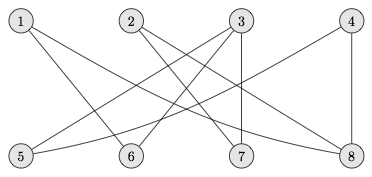
\includegraphics[width=\linewidth]{image/question3_matching.png}
        \end{column}
        
        \begin{column}{0.6\textwidth}
            \begin{block}{問題 (2)}
                $G_1$ の完全マッチングをすべて答えよ．
            \end{block}
            \textbf{【解法のロジック】}
            \begin{itemize}
                \item 頂点7の接続先は頂点2のみ $\Rightarrow$ $\{2, 7\}$ は必須．
                \item 頂点5の接続先は2と4だが，2が埋まったため $\{4, 5\}$ も必須．
                \item 残る頂点 $\{1, 3, 6, 8\}$ の組み合わせを検討．
            \end{itemize}
            
            \textbf{【解答】} 以下の2つ．
            \begin{enumerate}
                \item $M_1 = \{\{1, 6\}, \{2, 7\}, \{3, 8\}, \{4, 5\}\}$
                \item $M_2 = \{\{1, 8\}, \{2, 7\}, \{3, 6\}, \{4, 5\}\}$
            \end{enumerate}
        \end{column}
        
    \end{columns}
\end{frame}